\documentclass[12pt,a4paper]{article}

\usepackage[spanish]{babel}
\usepackage[utf8]{inputenc}
\usepackage[T1]{fontenc}
\usepackage{lmodern}
\usepackage{geometry}
\usepackage{setspace}
\usepackage{booktabs}
\usepackage{longtable}
\usepackage{array}
\usepackage{float}
\usepackage{graphicx}
\usepackage{amsmath,amssymb}
\usepackage[hidelinks]{hyperref}

\geometry{margin=2.5cm}
\onehalfspacing

\title{\textbf{Reporte de Estadística Inferencial en R}\\
\large Costos y presupuestos en salud}
\author{Mariana Soto Villada}
\date{\today}

\begin{document}

\maketitle
\tableofcontents
\newpage

\section{Introducción}
Este reporte presenta el análisis estadístico inferencial desarrollado en \texttt{R} a partir del conjunto de datos \textit{Medical Cost Personal Dataset} (\texttt{insurance.csv}), con el objetivo de estudiar factores asociados al costo anual del seguro médico (\texttt{costo\_anual}). El trabajo se organizó siguiendo la guía del curso: análisis descriptivo, pruebas de hipótesis, correlación, regresión lineal múltiple e inferencia/predicción.

El conjunto original contiene 1338 observaciones. Como la actividad exige trabajar con 70 registros, se implementó un muestreo estratificado proporcional para conservar representatividad en variables cualitativas clave.

La base de datos fue tomada de un repositorio público de referencia para práctica estadística y se cita formalmente en la sección de referencias, siguiendo la recomendación académica de uso de norma APA.

\section{Planteamiento del problema e hipótesis}
\textbf{Problema de estudio:} determinar qué variables demográficas y de hábitos de vida se asocian con incrementos en el costo anual del seguro médico y evaluar si esas asociaciones son estadísticamente significativas.

\textbf{Hipótesis general:}
\begin{itemize}
    \item \(H_0\): no existe relación estadísticamente significativa entre las variables explicativas (edad, IMC, número de hijos, sexo, hábito de fumar y región) y el costo anual del seguro.
    \item \(H_1\): existe al menos una relación estadísticamente significativa entre las variables explicativas y el costo anual del seguro.
\end{itemize}

\section{Descripción de datos y diseño muestral}
\subsection{Dataset original}
El dataset inicial incluye 7 variables:
\begin{itemize}
    \item Cuantitativas: edad, IMC, número de hijos, costo anual.
    \item Cualitativas: sexo, condición de fumador, región.
\end{itemize}

Resumen general reportado en el notebook:
\begin{itemize}
    \item \(n=1338\) observaciones.
    \item Edad: min \(=18\), media \(\approx 39.21\), max \(=64\).
    \item IMC: media \(\approx 30.66\).
    \item Costo anual: media \(\approx 13270\), mediana \(\approx 9382\), max \(\approx 63770\).
\end{itemize}

\subsection{Muestreo estratificado proporcional (70 casos)}
Se estratificó por la combinación condición de fumador \(\times\) región. Posteriormente, se ajustó el redondeo para obtener exactamente 70 observaciones.

\begin{table}[H]
\centering
\caption{Asignación muestral proporcional por estrato}
\begin{tabular}{llrrrr}
\toprule
\textbf{Fumador} & \textbf{Región} & \(\mathbf{N_{total}}\) & \(\mathbf{p}\) & \(\mathbf{n_{raw}}\) & \(\mathbf{n_{sample}}\) \\
\midrule
No  & Noreste & 257 & 0.1921 & 13.45 & 13 \\
No  & Noroeste & 267 & 0.1996 & 13.97 & 14 \\
No  & Sureste & 273 & 0.2040 & 14.28 & 14 \\
No  & Suroeste & 267 & 0.1996 & 13.97 & 14 \\
Sí & Noreste & 67  & 0.0501 & 3.51  & 4 \\
Sí & Noroeste & 58  & 0.0433 & 3.03  & 3 \\
Sí & Sureste & 91  & 0.0680 & 4.76  & 5 \\
Sí & Suroeste & 58  & 0.0433 & 3.03  & 3 \\
\bottomrule
\end{tabular}
\end{table}

\noindent Verificación: \(\sum n_{sample}=70\).

\subsection{Comparación de composición: original vs muestra}
\begin{table}[H]
\centering
\caption{Proporción por hábito de fumar}
\begin{tabular}{lrr}
\toprule
\textbf{Grupo} & \textbf{Original} & \textbf{Muestra 70} \\
\midrule
No fumador & 0.7952 & 0.7857 \\
Fumador    & 0.2048 & 0.2143 \\
\bottomrule
\end{tabular}
\end{table}

\begin{table}[H]
\centering
\caption{Proporción por región}
\begin{tabular}{lrr}
\toprule
\textbf{Región} & \textbf{Original} & \textbf{Muestra 70} \\
\midrule
Noreste & 0.2422 & 0.2429 \\
Noroeste & 0.2429 & 0.2429 \\
Sureste & 0.2720 & 0.2714 \\
Suroeste & 0.2429 & 0.2429 \\
\bottomrule
\end{tabular}
\end{table}

Las proporciones son muy similares, lo que respalda que la reducción a 70 casos conserva estructura poblacional en variables categóricas relevantes.

\section{Variables para requisitos de la actividad}
En la muestra final se trabajó con:
\begin{itemize}
    \item Cuantitativas continuas: IMC, costo anual.
    \item Cuantitativa discreta: número de hijos.
    \item Cualitativas nominales: sexo, condición de fumador.
    \item Cualitativa ordinal derivada: nivel de riesgo (Bajo, Medio, Alto).
\end{itemize}
Además se mantuvieron edad y región para enriquecer el análisis.

\section{Análisis descriptivo}
\subsection{Estadísticos principales}
\begin{table}[H]
\centering
\caption{Resumen descriptivo en la muestra de 70}
\begin{tabular}{lrrrrrr}
\toprule
\textbf{Variable} & \textbf{Media} & \textbf{DE} & \textbf{Mediana} & \textbf{Mínimo} & \textbf{Máximo} \\
\midrule
Edad      & 40.31 & 13.47 & ---      & 18.00   & 64.00 \\
IMC       & 31.39 & 4.78  & ---      & 20.23   & 41.33 \\
Número de hijos & 1.30  & 1.31  & ---      & 0       & 5 \\
Costo anual  & 14986.02 & 13819.74 & 10319.29 & 1121.87 & 60021.40 \\
\bottomrule
\end{tabular}
\end{table}

\subsection{Visualizaciones descriptivas}
\begin{figure}[H]
\centering
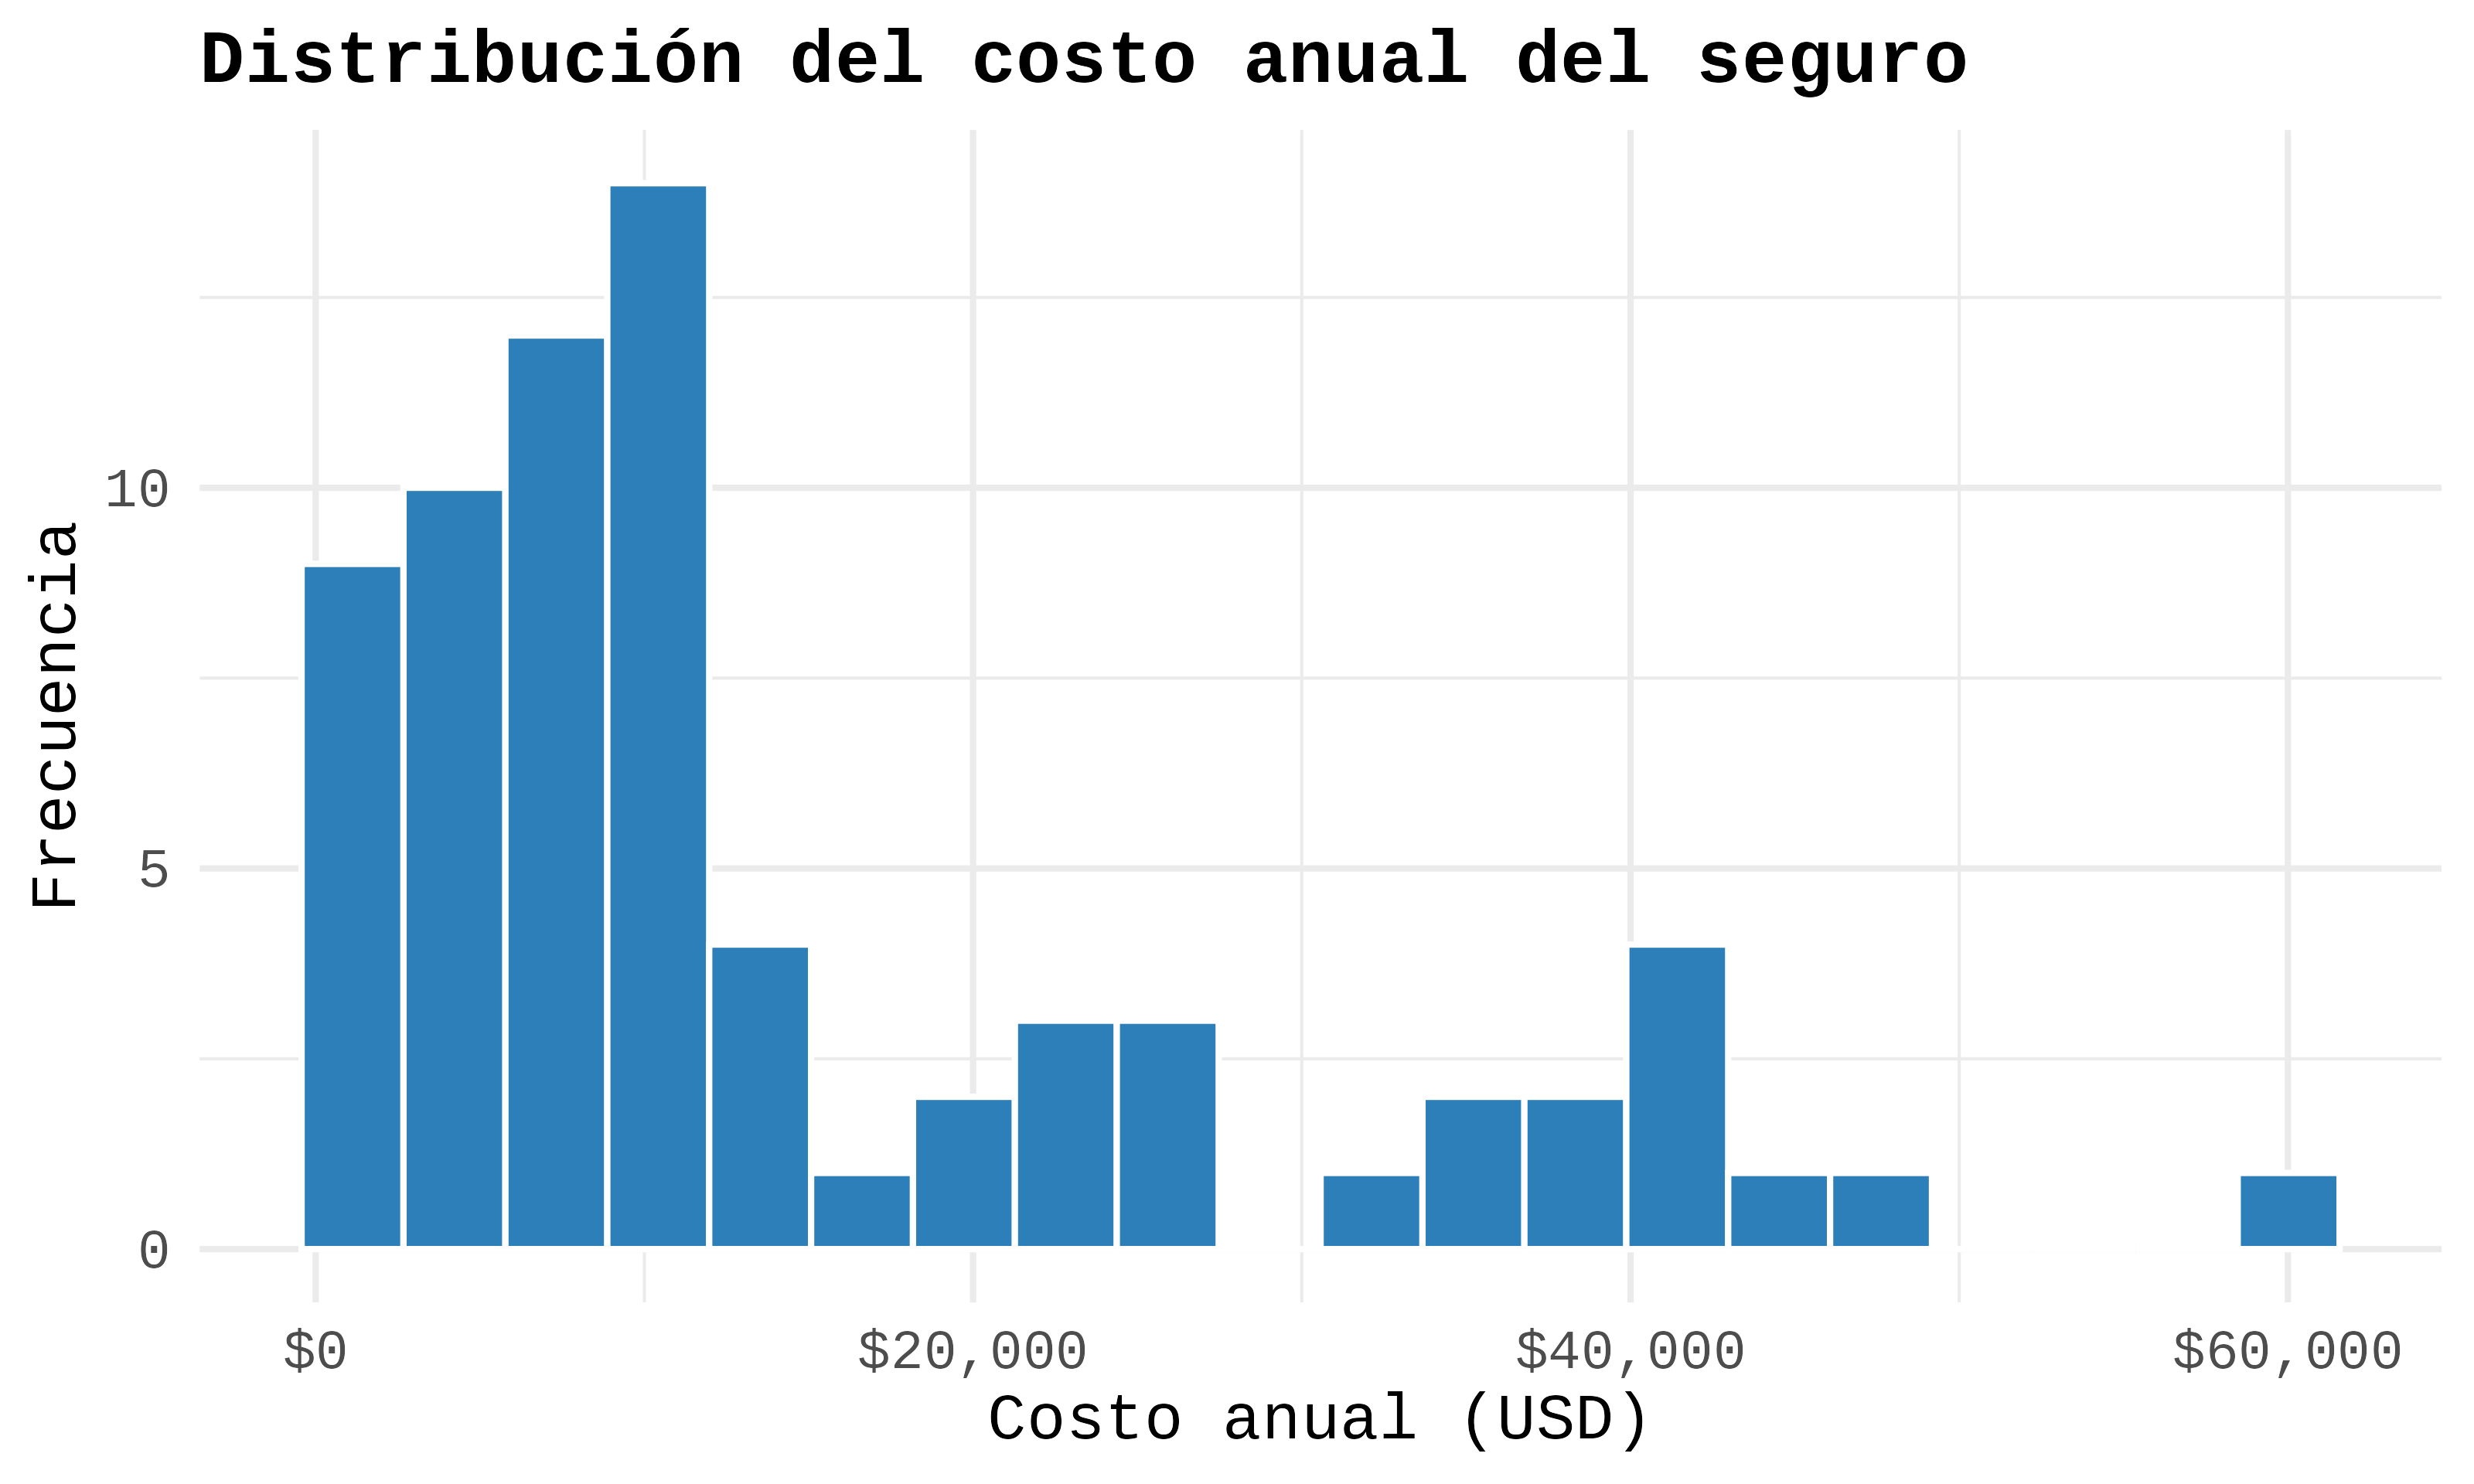
\includegraphics[width=0.95\textwidth]{figuras_reporte/histograma_costo_anual.png}
\caption{Distribución del costo anual del seguro.}
\label{fig:hist_charges}
\end{figure}

\begin{figure}[H]
\centering
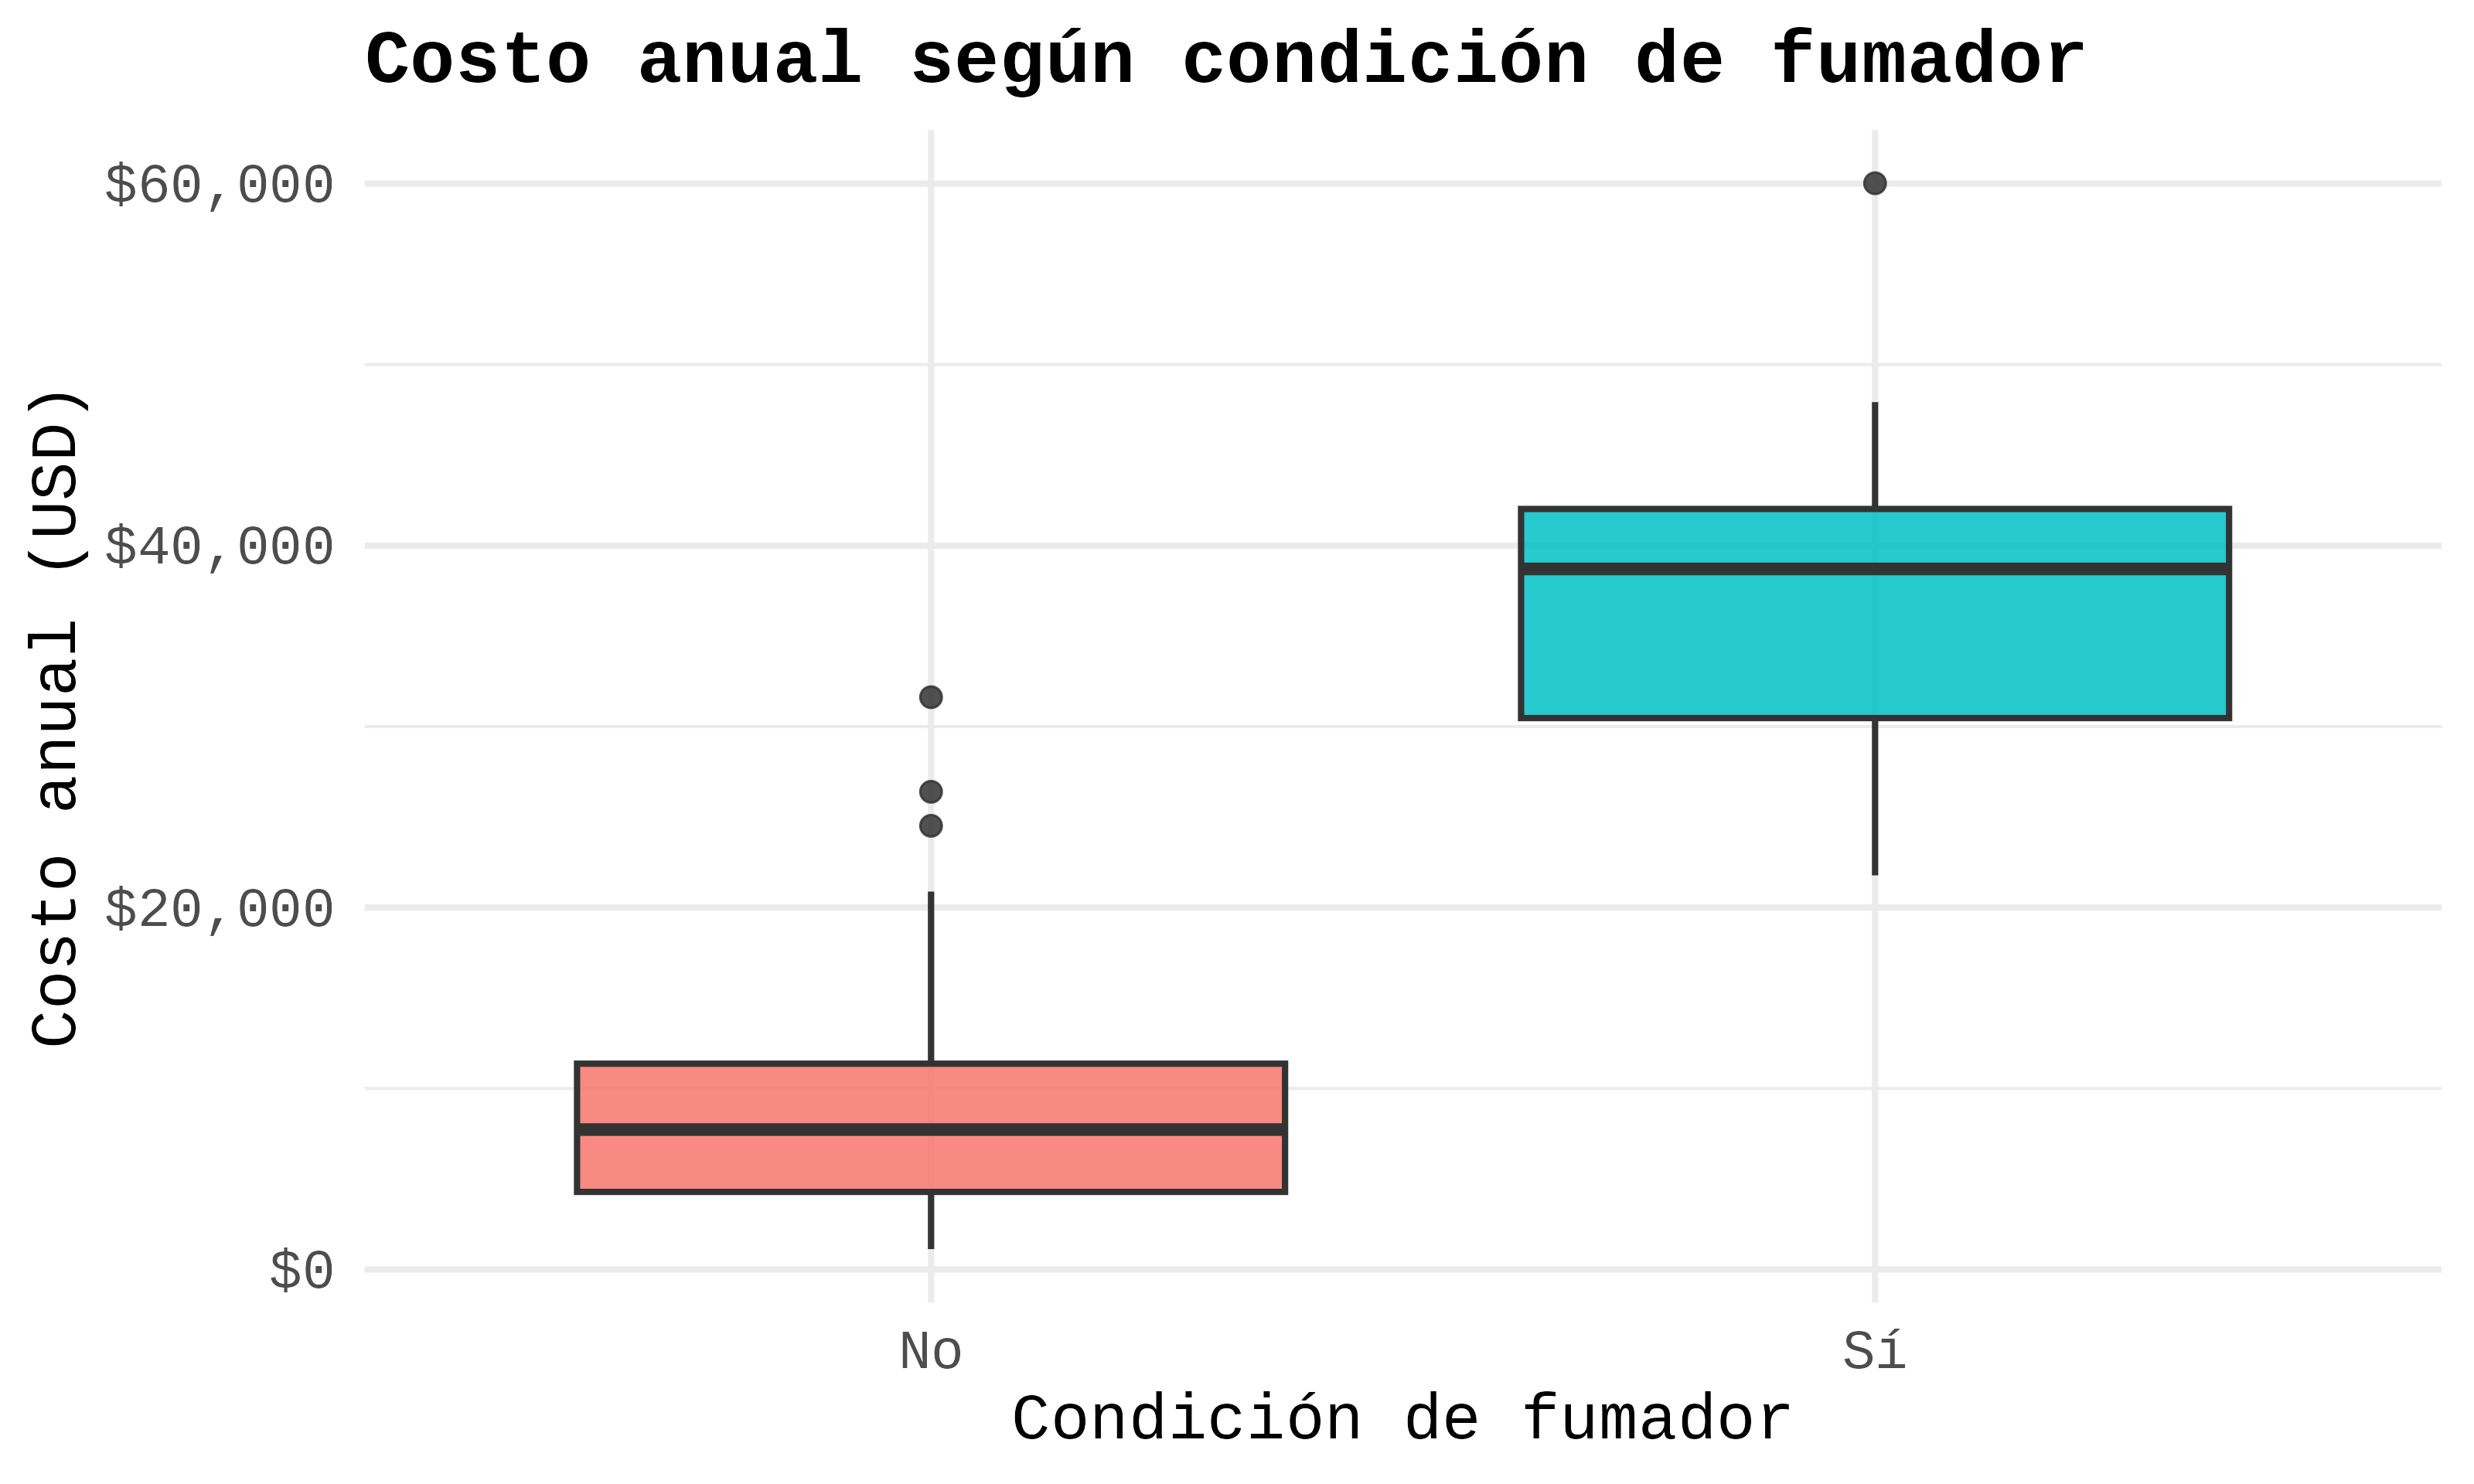
\includegraphics[width=0.95\textwidth]{figuras_reporte/boxplot_costo_por_fumador.png}
\caption{Comparación del costo anual entre fumadores y no fumadores.}
\label{fig:box_smoker}
\end{figure}

\begin{figure}[H]
\centering
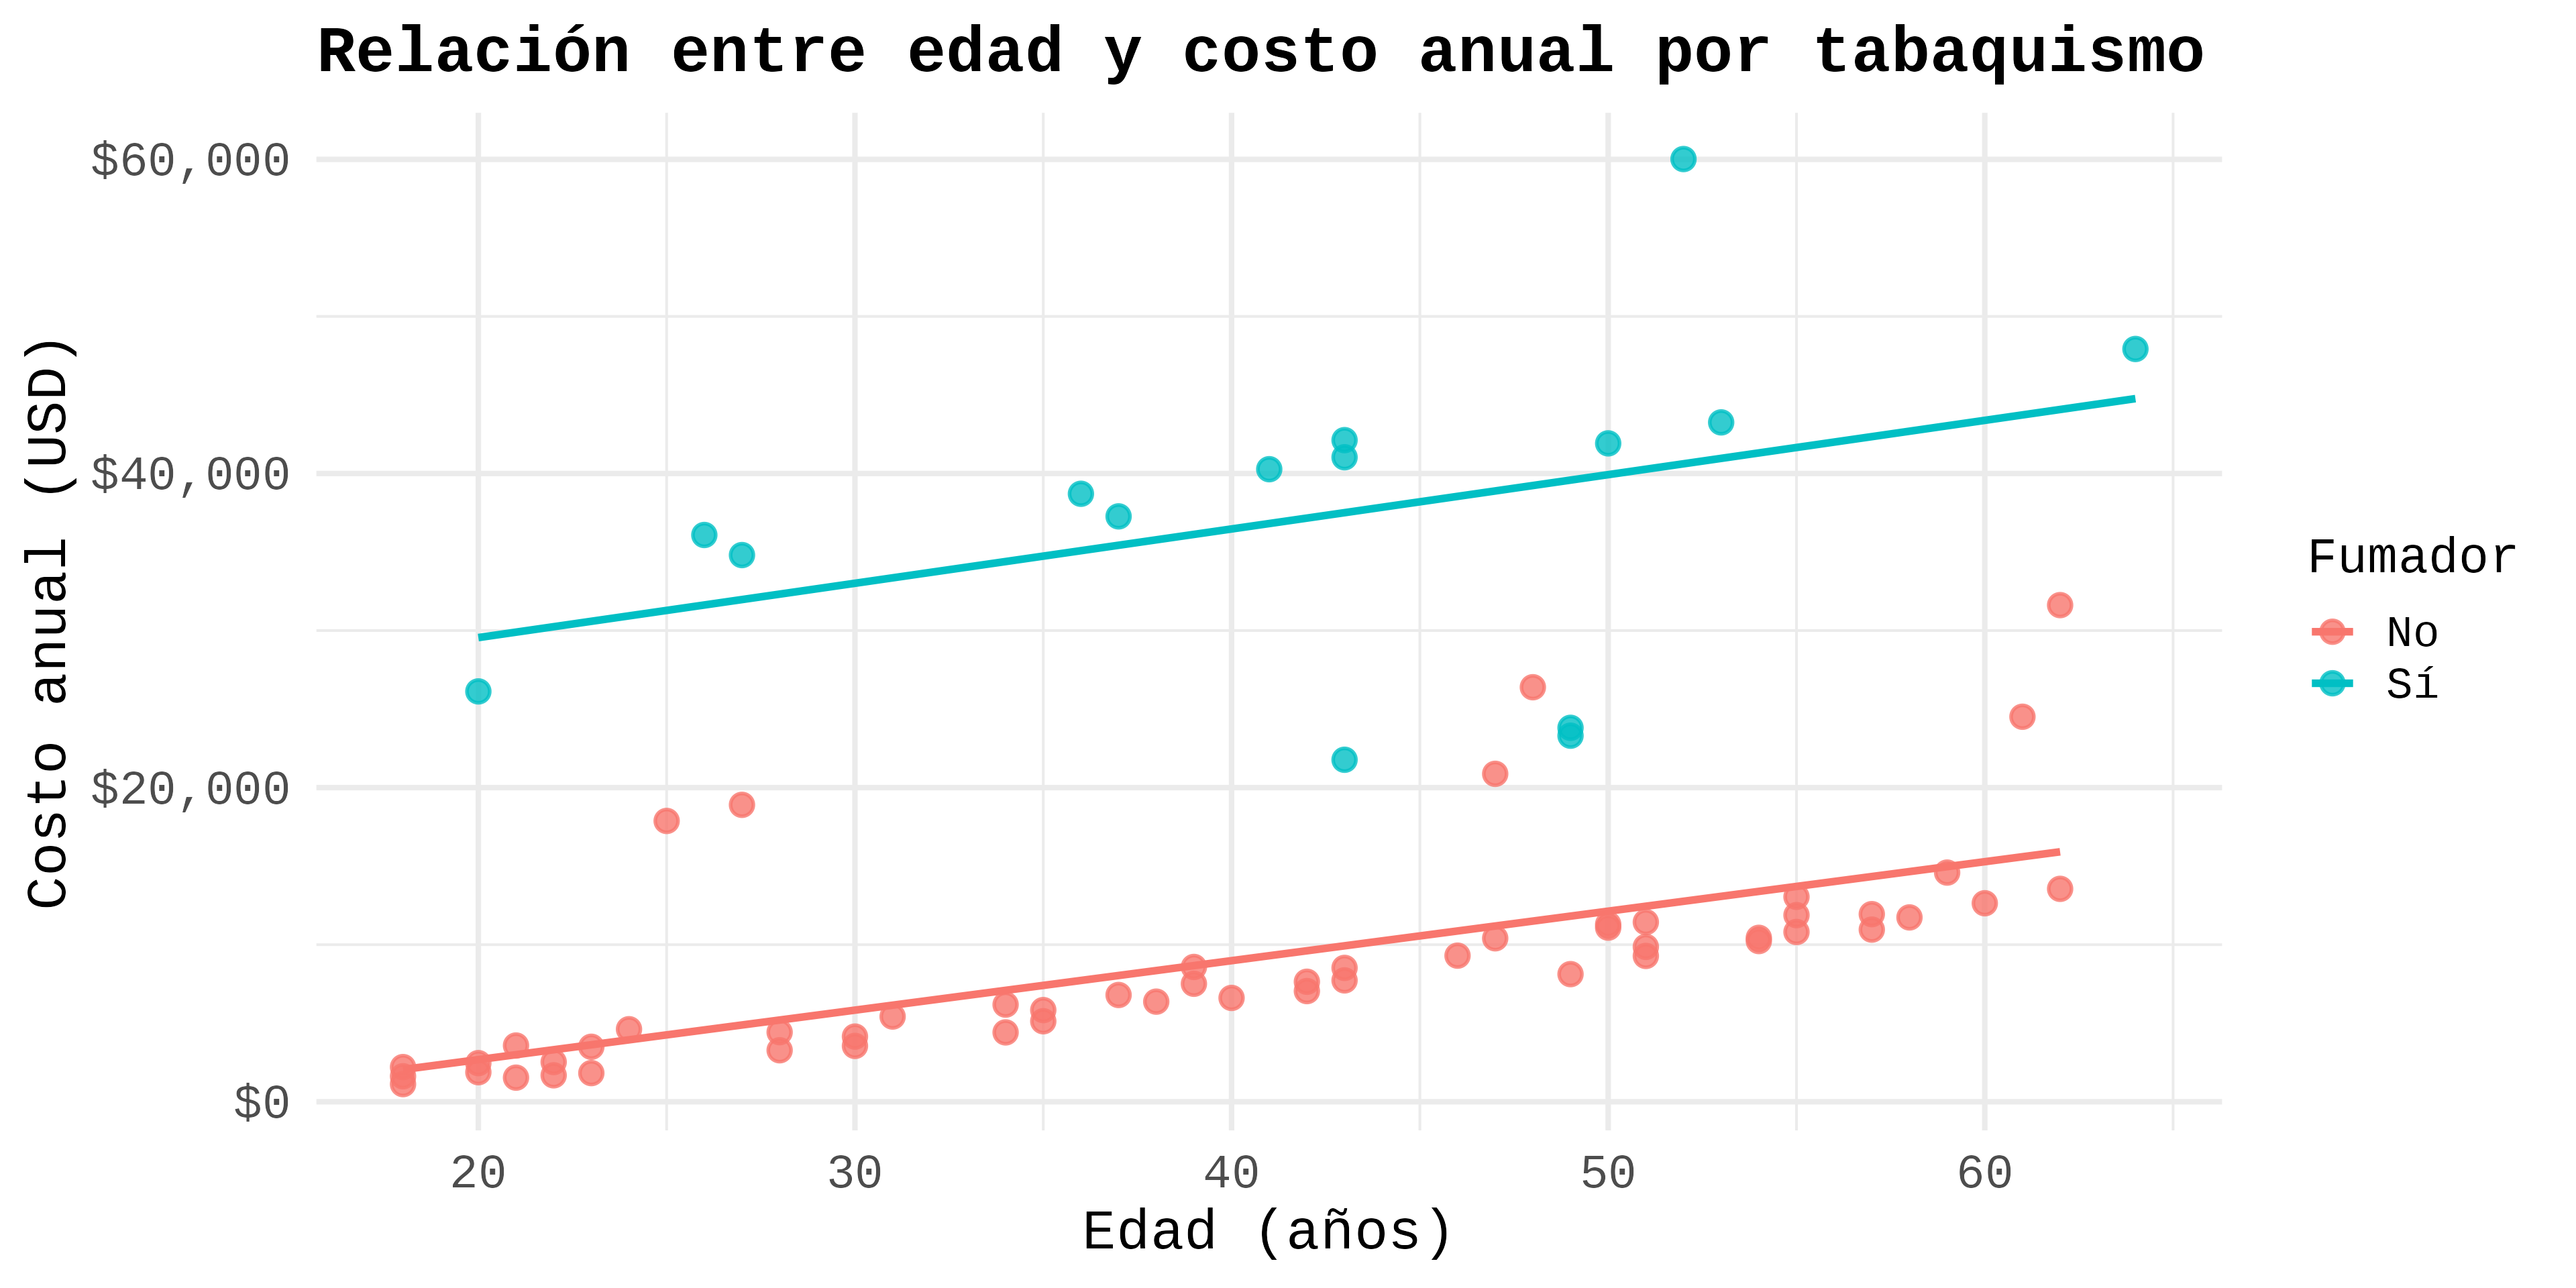
\includegraphics[width=0.95\textwidth]{figuras_reporte/dispersion_edad_costo_anual.png}
\caption{Relación entre edad y costo anual según condición de fumador.}
\label{fig:scatter_age_charges}
\end{figure}

\subsection{Interpretación descriptiva}
\begin{enumerate}
    \item El costo anual presenta asimetría positiva: pocos individuos concentran costos muy altos.
    \item Los fumadores tienden a exhibir costos superiores a los no fumadores.
    \item Se observa tendencia creciente entre edad y costo, especialmente en fumadores.
\end{enumerate}

\section{Pruebas de hipótesis (\(\alpha=0.05\))}
\begin{table}[H]
\centering
\caption{Resultados inferenciales principales}
\begin{tabular}{p{4cm}p{5cm}p{4cm}p{2cm}}
\toprule
\textbf{Prueba} & \textbf{Hipótesis nula} & \textbf{Resultado} & \textbf{Decisión} \\
\midrule
Shapiro--Wilk sobre costo anual & La distribución es normal & \(W=0.82673,\; p=1.322\times 10^{-7}\) & Rechazar \(H_0\) \\
\addlinespace
Chi-cuadrado (sexo vs fumador) & Independencia entre variables & \(\chi^2=4.5372,\; gl=1,\; p=0.03317\) & Rechazar \(H_0\) \\
\addlinespace
t de Welch (IMC por sexo) & Igualdad de medias de IMC & \(t=-0.16483,\; p=0.8696\) & No rechazar \(H_0\) \\
\addlinespace
Mann--Whitney (costo anual por fumador) & Igualdad de distribución/localización & \(W=11,\; p=9.492\times 10^{-9}\) & Rechazar \(H_0\) \\
\bottomrule
\end{tabular}
\end{table}

\noindent \textbf{Síntesis:} los costos no siguen normalidad en la muestra, hay evidencia de asociación entre sexo y hábito de fumar, no hay evidencia de diferencia de IMC promedio por sexo, y sí hay una diferencia marcada de costos entre fumadores y no fumadores.

\section{Correlación y regresión lineal múltiple}
\subsection{Correlación de Pearson}
\begin{table}[H]
\centering
\caption{Matriz de correlación (variables numéricas)}
\begin{tabular}{lrrrr}
\toprule
\textbf{Variable} & \textbf{Edad} & \textbf{IMC} & \textbf{N.º hijos} & \textbf{Costo anual} \\
\midrule
Edad      & 1.000 & -0.049 & 0.141 & 0.372 \\
IMC       & -0.049 & 1.000 & -0.078 & 0.161 \\
Hijos     & 0.141 & -0.078 & 1.000 & 0.016 \\
Costo anual  & 0.372 & 0.161 & 0.016 & 1.000 \\
\bottomrule
\end{tabular}
\end{table}

\subsection{Modelo de regresión}
Se estimó:
\[
\texttt{costo\_anual} \sim \texttt{edad}+\texttt{imc}+\texttt{hijos}+\texttt{fumador}+\texttt{sexo}+\texttt{region}.
\]

\begin{table}[H]
\centering
\caption{Coeficientes del modelo lineal múltiple}
\begin{tabular}{lrrrr}
\toprule
\textbf{Término} & \textbf{Estimación} & \textbf{Error estándar} & \textbf{t} & \textbf{p-valor} \\
\midrule
Intercept          & -12071.39 & 5275.43 & -2.288 & 0.0256 \\
Edad                & 322.98    & 50.24   & 6.429  & \(2.2\times10^{-8}\) \\
IMC                 & 379.96    & 138.56  & 2.742  & 0.0080 \\
Número de hijos     & 392.52    & 508.57  & 0.772  & 0.4432 \\
Fumador (Sí)        & 27743.07  & 1651.18 & 16.802 & \(<2\times10^{-16}\) \\
Sexo (Hombre)       & -1582.95  & 1360.86 & -1.163 & 0.2493 \\
Región (Noroeste)   & -5119.10  & 1916.69 & -2.671 & 0.0097 \\
Región (Sureste)    & -3728.34  & 1845.25 & -2.021 & 0.0477 \\
Región (Suroeste)   & -5627.17  & 1872.51 & -3.005 & 0.0038 \\
\bottomrule
\end{tabular}
\end{table}

\noindent Estadísticos globales del ajuste:
\begin{itemize}
    \item Error estándar residual: 5380 (61 g.l.).
    \item \(R^2 = 0.866\), \(R^2\) ajustado \(=0.8485\).
    \item Prueba F global: \(F(8,61)=49.29,\; p<2.2\times10^{-16}\).
\end{itemize}

\subsection{Lectura del modelo}
\begin{itemize}
    \item La condición de fumador (Sí) es el predictor con mayor impacto: incrementa fuertemente el costo esperado.
    \item Edad e IMC también aportan incrementos significativos en costos.
    \item Número de hijos y sexo (Hombre) no resultaron significativos al \(5\%\) en este ajuste.
    \item El modelo explica una proporción alta de variabilidad del costo (\(R^2\) elevado).
\end{itemize}

\subsection{Diagnóstico de supuestos}
\begin{figure}[H]
\centering
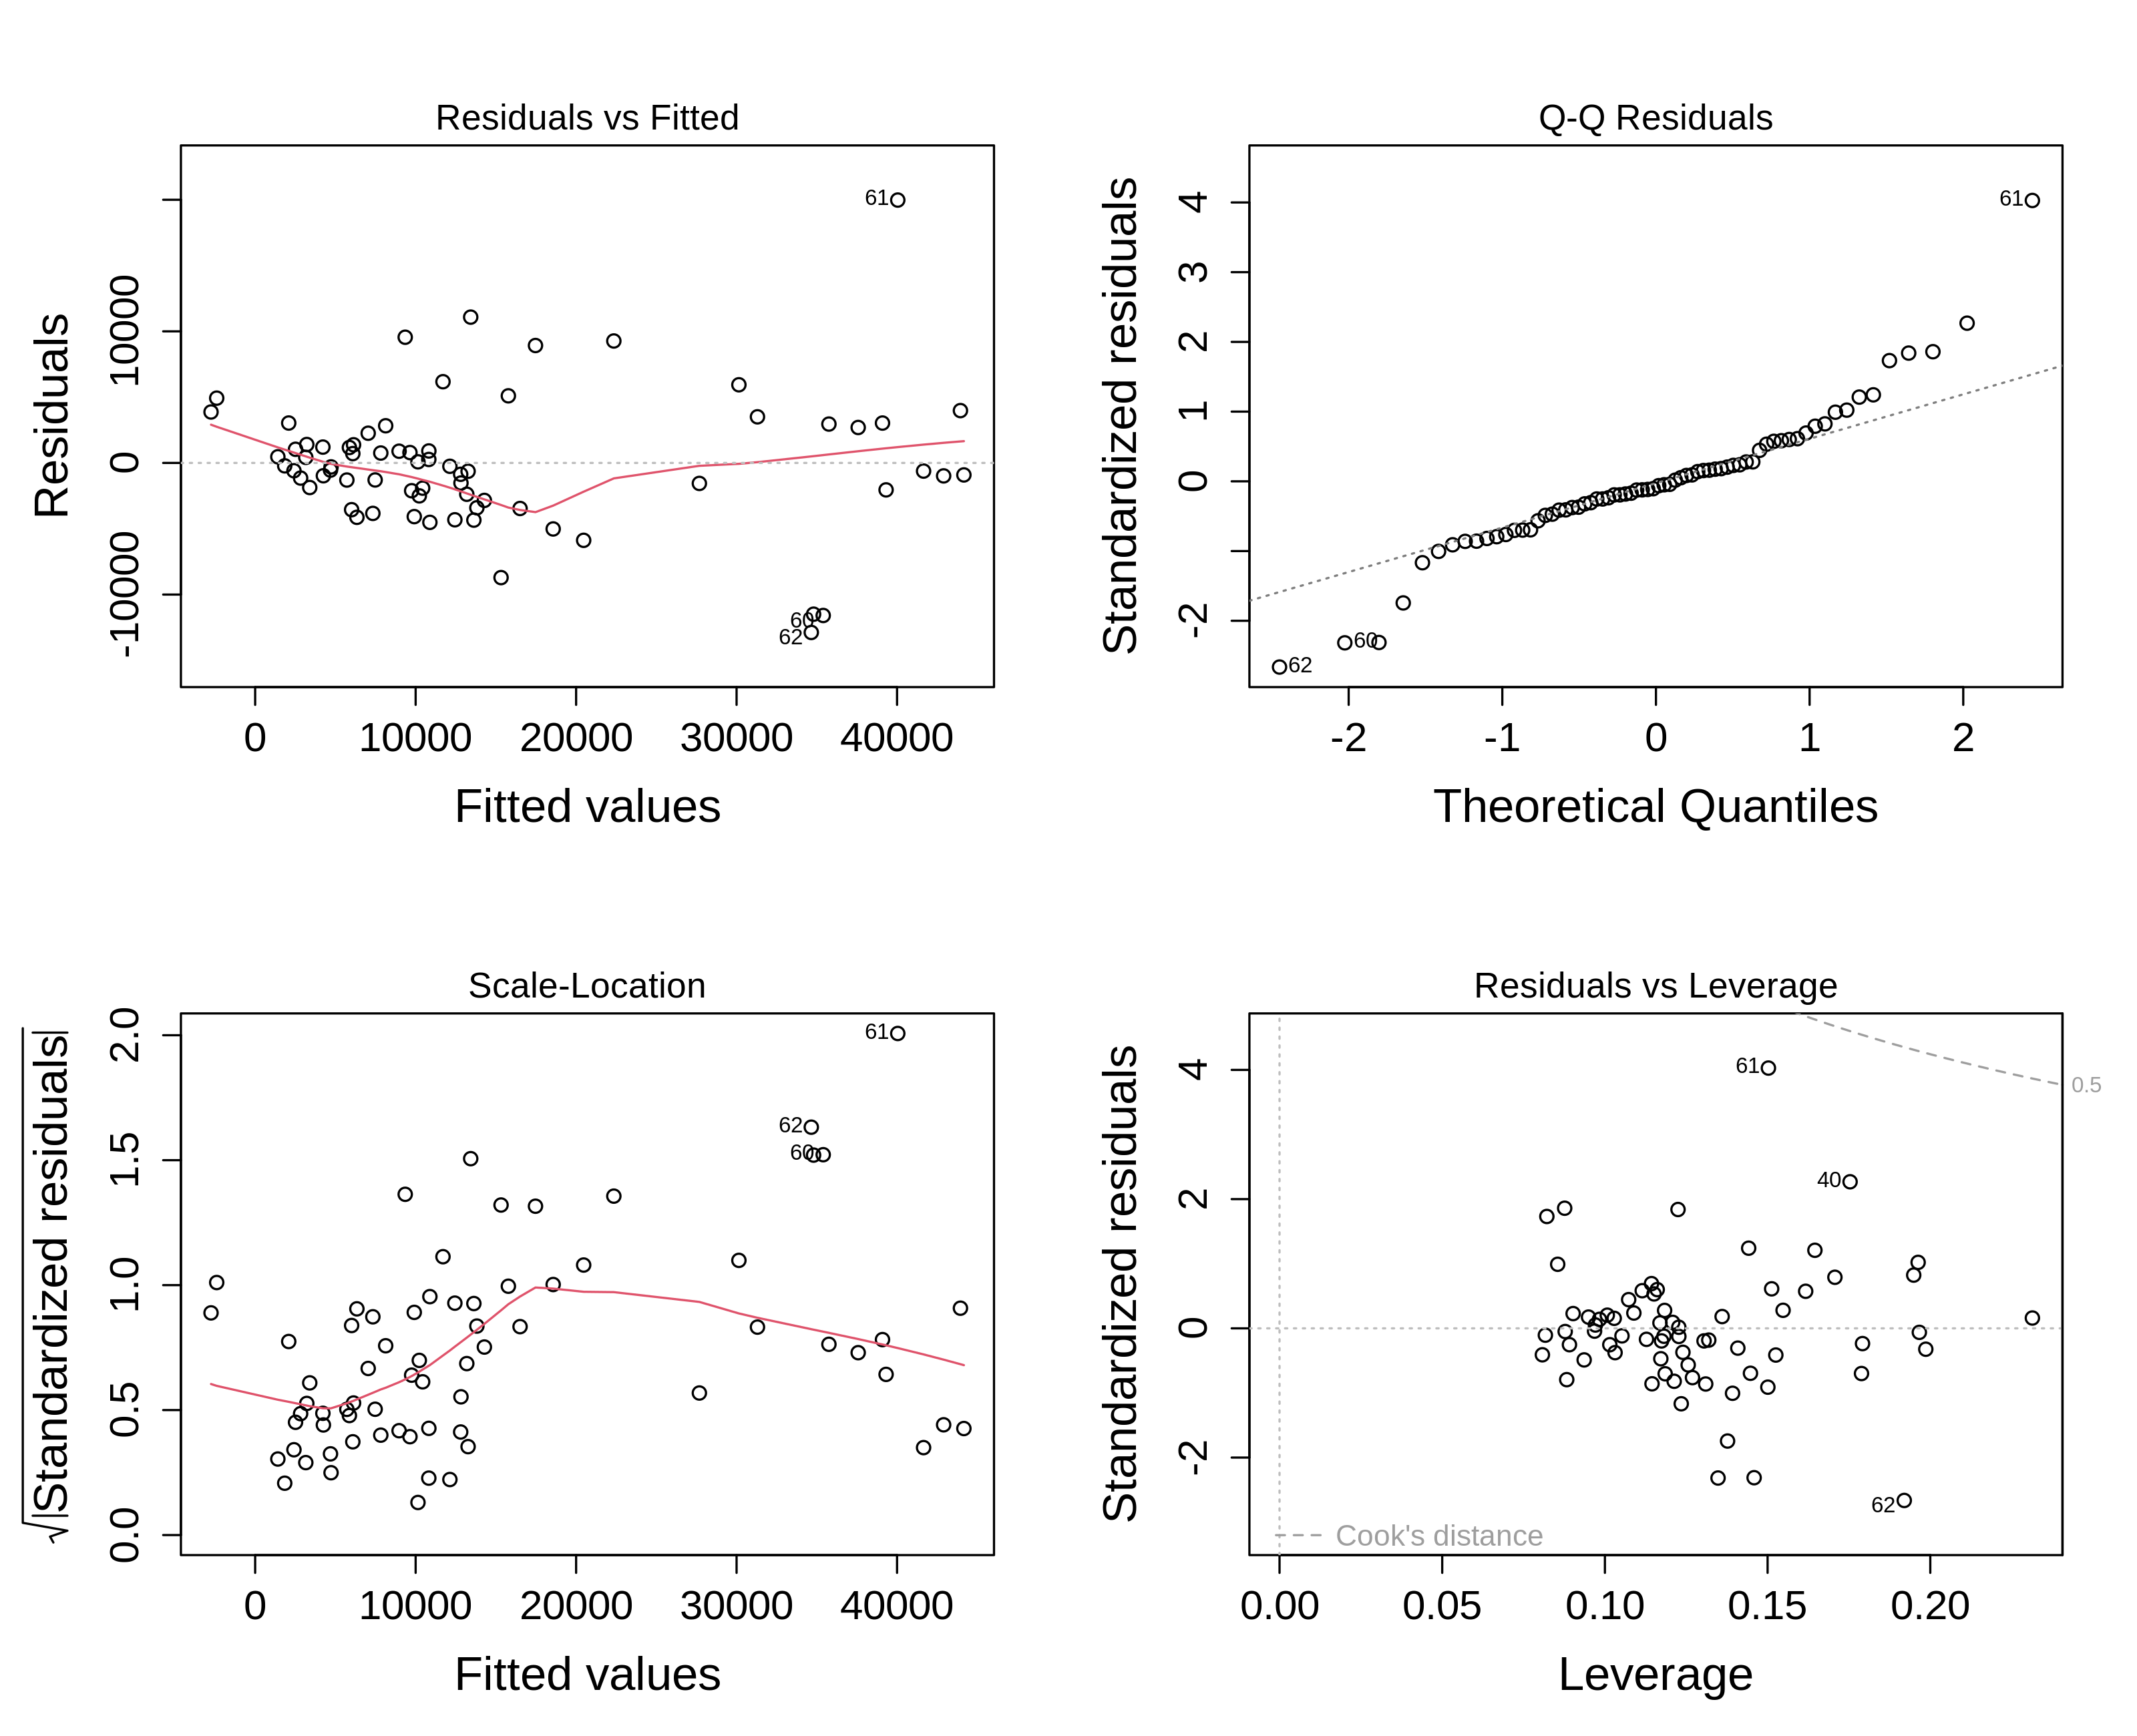
\includegraphics[width=0.95\textwidth]{figuras_reporte/diagnostico_modelo_regresion.png}
\caption{Diagnóstico de linealidad, homocedasticidad, normalidad de residuos e influencia.}
\label{fig:diag_modelo}
\end{figure}

\section{Inferencia y predicción}
Se evaluaron predicciones para tres perfiles:
\begin{table}[H]
\centering
\caption{Predicción puntual e intervalo de predicción (\texttt{predict(..., interval = "prediction")} en R). El caso marcado con \(^{\dagger}\) debe interpretarse como costo cercano a cero, no literal.}
\begin{tabular}{rrrrllrrr}
\toprule
\textbf{Edad} & \textbf{IMC} & \textbf{Hijos} & \textbf{Fumador} & \textbf{Sexo} & \textbf{Región} & \textbf{Predicción} & \textbf{Límite inferior} & \textbf{Límite superior} \\
\midrule
25 & 24 & 0 & No  & Mujer & Noroeste & 2.93\(^{\dagger}\)    & -11509.87\(^{\dagger}\) & 11515.74 \\
45 & 30 & 2 & Sí & Hombre   & Sureste & 37078.18 & 25714.43  & 48441.93 \\
60 & 33 & 3 & No  & Mujer & Noreste & 21023.48 & 9604.75   & 32442.21 \\
\bottomrule
\end{tabular}
\end{table}
\noindent{\footnotesize \(^{\dagger}\) Valor transcrito del notebook. En modelos lineales con respuesta positiva y asimétrica, pueden aparecer predicciones no factibles; este caso se interpreta como costo esperado muy bajo (cercano a cero), no como monto literal.}

\noindent \textbf{Nota de interpretación:} el primer perfil presenta una predicción puntual muy baja y un límite inferior negativo. Esto no implica un costo real negativo, sino una limitación conocida del modelo lineal gaussiano cuando la variable respuesta es estrictamente positiva y altamente asimétrica.

\noindent El intervalo de predicción es amplio porque incorpora variabilidad individual; por ello es más útil para planeación presupuestal que una sola estimación puntual. En una extensión metodológica, conviene evaluar modelos con transformación \(\log(\texttt{costo\_anual})\) o alternativas con restricción de positividad.

\section{Conclusiones}
\begin{enumerate}
    \item El muestreo estratificado proporcional permitió cumplir el requisito de 70 observaciones con buena representatividad de subgrupos.
    \item El costo anual de salud muestra alta dispersión y asimetría positiva.
    \item Ser fumador está fuertemente asociado a incrementos del costo médico, tanto descriptiva como inferencialmente.
    \item El modelo lineal múltiple presentó buen ajuste global (\(R^2=0.866\)) y confirmó la relevancia de edad, IMC y tabaquismo.
    \item El enfoque aplicado aporta evidencia cuantitativa para decisiones en costos y presupuestos de salud.
\end{enumerate}

\section{Referencias}
\begin{itemize}
    \item stedy. (s.\,f.). \textit{Machine-Learning-with-R-datasets} [Conjunto de datos \texttt{insurance.csv}]. GitHub. \url{https://github.com/stedy/Machine-Learning-with-R-datasets}. Recuperado el 10 de mayo de 2026.
    \item Instituto Tecnológico Metropolitano. (2026). \textit{Guía de trabajo de campo: Estadística inferencial en Excel o RStudio}. Material del curso de Estadística.
\end{itemize}


\end{document}
